% Template for PLoS
% Version 1.0 January 2009
%
% To compile to pdf, run:
% latex plos.template
% bibtex plos.template
% latex plos.template
% latex plos.template
% dvipdf plos.template

\documentclass[10pt]{article}

% amsmath package, useful for mathematical formulas
\usepackage{amsmath}
% amssymb package, useful for mathematical symbols
\usepackage{amssymb}

% graphicx package, useful for including eps and pdf graphics
% include graphics with the command \includegraphics
\usepackage{graphicx}

% cite package, to clean up citations in the main text. Do not remove.
\usepackage{cite}

\usepackage{color}

% Use doublespacing - comment out for single spacing
%\usepackage{setspace}
%\doublespacing
\usepackage{lineno}
\linenumbers

\newcommand{\argmin}{\operatornamewithlimits{argmin}}

% Text layout
\topmargin 0.0cm
\oddsidemargin 0.5cm
\evensidemargin 0.5cm
\textwidth 16cm
\textheight 21cm

% Bold the 'Figure #' in the caption and separate it with a period
% Captions will be left justified
\usepackage[labelfont=bf,labelsep=period,justification=raggedright]{caption}

% Use the PLoS provided bibtex style
\bibliographystyle{plos2009}

% Remove brackets from numbering in List of References
\makeatletter
\renewcommand{\@biblabel}[1]{\quad#1.}
\makeatother


% Leave date blank
\date{}

\pagestyle{myheadings}
%% ** EDIT HERE **


%% ** EDIT HERE **
%% PLEASE INCLUDE ALL MACROS BELOW

%% END MACROS SECTION

\begin{document}

% Title must be 150 characters or less
\begin{flushleft}
{\Large
\textbf{PhyloSift: phylogenetic analysis of genomes and metagenomes}
}
% Insert Author names, affiliations and corresponding author email.
\\
Aaron E. Darling$^{1,\ast}$,
Guillaume Jospin$^{1}$,
Eric Lowe$^{1}$,
Frederick A. Matsen IV$^{4}$,
Holly M. Bik$^{1}$,
Jonathan A. Eisen$^{2,3}$
\\
\bf{1} Genome Center, University of California, Davis, California, United States of America
\\
\bf{2} Department of Evolution and Ecology, University of California, Davis, California, United States of America
\\
\bf{3} Department of Medical Microbiology and Immunology, University of California, Davis, California, United States of America
\\
\bf{4} Fred Hutchinson Cancer Research Center, Seattle, Washington, United States of America
\\
$\ast$ E-mail: aarondarling@ucdavis.edu
\end{flushleft}

% % Please keep the abstract between 250 and 300 words
% \section*{Abstract}
% Like all organisms on the planet, environmental microbes are subject to the forces of molecular evolution.
% Metagenomic sequencing provides a means to access the DNA sequence of uncultured microbes.
% By combining DNA sequencing of microbial communities with evolutionary modeling and phylogenetic analysis we might obtain new insights into microbiology and also provide a basis for practical tools such as forensic pathogen detection.

% In this work we present an approach to leverage phylogenetic analysis of metagenomic sequence data to conduct several types of analysis.
% First, we present a method to conduct phylogeny-driven Bayesian hypothesis tests for the presence of an organism in a sample.
% Second, we present a means to compare community structure across a collection of many samples and develop direct associations between the abundance of certain organisms and sample metadata.
% Third, we apply new tools to analyze the phylogenetic diversity of microbial communities and again demonstrate how this can be associated to sample metadata.

% These analyses are implemented in an open source software pipeline called PhyloSift.
% As a pipeline, PhyloSift incorporates several other programs including LAST, HMMER, and pplacer to automate phylogenetic analysis of protein coding and RNA sequences in metagenomic datasets generated by modern sequencing platforms (e.g. Illumina, 454).


% % Please keep the Author Summary between 150 and 200 words
% % Use first person. PLoS ONE authors please skip this step.
% % Author Summary not valid for PLoS ONE submissions.
% \section*{Author Summary}

\clearpage

\section*{Introduction}

Metagenomics - the sequencing of DNA isolated directly from the environment - has quickly become a routinely used tool with wide application~\cite{thomas2012metagenomics}. Used primarily in the study of microorganisms, metagenome sequencing has now been carried out on a variety of environments where one finds microbes - from plants and animals to every kind of natural and man-made environment around the globe.
Metagenomic sequencing has provided fundamental insight into the diversity of microbes and their function and roles in ecosystems.
Initially, metagenomics was used largely as a way of simply obtaining some genomic information about organisms that were not cultured (i.e., nobody had figured out how to grow them in isolation in a controlled environment) (e.g., \cite{beja2000bacterial}).
However, due to decreases in the cost and the difficulty of sequencing, metagenomics has become a tool for studying any microbial community, regardless of cultivability.

One strength of metagenomic approaches arises from the ability to sample the genomes of organisms in a particular environment approximately uniformly at random.  This effect is achieved with the random ``shotgun'' sequencing methods originally applied for \textit{de novo} genomes sequencing of individual organisms~\cite{venter2004environmental,tyson2004community}.
From random shotgun sequence data of DNA isolated from environmental samples, one can make inferences about what organisms are present in a sample (i.e., who is there?) as well as what is their functional potential (i.e., what are they doing?).
In addition, by comparing shotgun metagenomic data across samples one can study larger scale issues such as ecology and biogeography and also attempt to correlate particular organisms or functions with ``metadata'' about samples (e.g., health status, nutrient cycling rates, etc) (e.g.\cite{tringe2005comparative}).
Furthermore, by sampling a community directly one can avoid certain problems inherent in culturing such as contamination, population bottlenecking, and taxonomic bias~\cite{eisen2007environmental}.  In this sense metagenomics can be considered an extension of ``culture-independent'' ribosomal RNA gene surveys~\cite{hugenholtz1998impact}. 
The great potential for novel insight into microbial communities has led researchers in diverse fields from medicine to agriculture, law enforcement, biodefense, ecology, evolution, and industry to apply metagenomic methods.

Athough great potential exists for metagenomics to yield insight into the hidden world of microbes, many challenges remain before this potential can be realized.
Perhaps the biggest challenges lie in analysis of the data~\cite{chen2005bioinformatics}.
First, metagenomic samples reflect entire communities of organisms, unlike ``traditional'' genome sequencing of individual organisms or clones (i.e., from cultures of a single isolate where genetic diversity has been bottlenecked).
The large number of microbial taxa in environmental samples can be a challenge for some types of analysis.
More vexing is when each species in a community is heterogenous with extensive genomic polymorphisms within the species~\cite{kunin2008bioinformatician}.
A related issue is that shotgun metagenomic sequencing protocols destroy some of the most valuable information present in a sample: genetic linkage.
Loss of linkage information occurs in two ways: during sample extraction and fragmentation of DNA for sequencing.
In nearly all metagenomic sample processing methods, cells from the microbial community are lysed together to obtain a common pool of DNA.
This practice causes DNA from many different cells to mix together, so that the cellular compartmentalization of individual genotypes is destroyed.
Subsequently, long chromosome-scale DNA fragments are typically broken by mechanical or enzymatic means into fragments small enough for processing with current sequencing protocols.
The resulting sequenced fragments are usually less than 1 Kbp in length.  Although it is possible to generate data for larger fragments via cloning~\cite{beja2000bacterial} or using Pacific Biosciences sequencing, most metagenomic data is currently being generated with short read/short insert sequencing chemistry such as that offered by Illumina.  Though short read methods are cheaper, quicker and easier than large fragment approaches, they come at a cost.  The shearing results in further loss of genetic linkage information, since we no longer have direct information on how short DNA fragments are arranged into chromosome-scale molecules.

The lack of linkage information limits the ability to use metagenomic data for evolutionary analysis, since most current methods assume complete linkage information is available.
In practice, improved sample processing methods could potentially retain the genetic linkage information of a microbial community throughout the sequencing process.
High throughput single-cell genomics (e.g. applied to thousands of cells) offers an alternative to the standard metagenomics workflow that preserves information about the compartmentalization of genetic material into cells ~\cite{Woyke2010,lasken2012genomic,rinke2013insights}
However, single cell approaches are still limited in their utility by a number of technical issues including contamination, expensive and extensive equipment needs, missing data, and the creation of chimeras~\cite{blainey2013future}; they will always be more limited in throughput than their standard metagenomics counterparts.

Thus the research community is left with developing and using computational methods to sift through and make sense of short read, random shotgun metagenomic data.
Though there are many important steps in analyzing metagenomic data, we believe that a critical component is phylogenetic analysis of the sequences.
Among the uses of phylogenetic analysis in metagenomics are: improved classification of sequences as to their taxonomic origin, functional prediction for genes, alternative metrics of alpha and beta diversity, improved identification of operational taxonomic units (OTUs), and sequence binning ~\cite{meyer2008metagenomics, Matsen2010, Evans2010, Kembel2011, Matsen2012, Stark2010, Wu2012, Brady2009, Brady2011, Sharpton2011, Jolley2012, sunagawa2013metagenomic}.

In the present manuscript, we introduce PhyloSift, a new method for phylogenetic analysis of metagenomic samples and for comparison of community structure among multiple related samples.
The new method leverages phylogenetic models of molecular evolution to provide high resolution detection of organisms in a metagenome.
Our approach is based on well known statistical phylogenetic models, is amenable to Bayesian hypothesis testing, and uses name-independent and OTU-free analyses to provide higher resolution about microbial community assemblages (versus methods that rely on taxonomy or OTUs).
These methods can be applied to any single phylogeny at a time, and expand on our previous experience building AMPHORA \cite{WuEisen2008}.
We additionally propose a set of 40 ``elite'' marker gene families that have largely congruent phylogenetic histories, thus improving the limit of detection for rare organisms in microbial communities.
We contribute an open-source implementation of the method that has been engineered for ease-of-use on 64-bit Linux and Mac platforms.
Finally, we compare the features of PhyloSift to some related methods to provide readers with insight into when use of our approach is and is not appropriate.


% You may title this section "Methods" or "Models".
% "Models" is not a valid title for PLoS ONE authors. However, PLoS ONE
% authors may use "Analysis"
\section*{Methods}

PhyloSift implements a method for analyzing microbial community structure directly from metagenome sequence data.
Figure~\ref{fig:overview} gives an overview of the analysis workflow as executed when analyzing a metagenomic sample.
The analysis can be decomposed into four stages: 1. searching input sequences for identity to a database of known reference gene families, 2. adding input sequences to a multiple alignment with reference genes, 3. placement of input sequences onto a phylogeny of reference genes, and 4. generation of taxonomic summaries. We now describe the details of each step along with our design decisions and rationale.


\subsection*{Reference gene families used by PhyloSift}

The standard PhyloSift database includes a set of 40 ``elite'' gene families previously identified as nearly universal among bacteria and archaea and in single-copy~\cite{DongyingWu2012}.
These ``elite'' families represent about 1\% of an average bacterial genome, as estimated from current genome databases.
In other work we have demonstrated that phylogenetic trees reconstructed on individual genes in this set are generally congruent with each other~\cite{Lang2012}, suggesting that concatenating alignments of these families will yield a valid and more powerful estimate of their phylogenetic history.
Other groups have also demonstrated that trees inferred from concatenate alignments demonstrate the least conflict with trees inferred separately from other microbial amino acid sequences~\cite{Abby2012}.
During the database update process (described below), these gene families are automatically extended to include putative homologs from eukarya and some viruses with large genomes such as the Mimivirus.
Most small viral genomes lack homologs of these gene families.

In addition to the elite 40 families, the PhyloSift database also includes four additional sets of gene families:
\begin{itemize}
\item 16S and 18s ribosomal {RNA} genes
\item mitochondrial gene families
\item Eukaryote-specific gene families
\item Viral gene families
\end{itemize}
Combined, this yields a set of approximately 800 gene families in the standard PhyloSift database, most of which are viral.

\subsection*{Detailed PhyloSift client workflow}
\subsubsection*{Sequence identity search}
This first step in a PhyloSift analysis aims to identify regions of the input sequences that may be homologous to gene families in the reference database.
Input sequences to this step can be of any length ranging from short 30nt next-generation sequence reads to fully assembled genomes or metagenomes.
Recognized input formats include FastA and FastQ (paired, unpaired, phred33, phred64, and/or interleaved pairing), and these can optionally be supplied as bzip2 or gzip compressed data files.
Sequence input can be streamed via stdin or unix named pipes.
Amino acid input sequences can also be processed.

PhyloSift uses LAST~\cite{Kiełbasa2011} for sequence similarity search against the reference databases.
We evaluated many possible search algorithms and implementations before finally selecting LAST.
Other options we evaluated were BLAST~\cite{Altschul1997}, BLAST+~\cite{Camacho2009}, and RAPsearch2~\cite{Zhao2011}, and bowtie2~\cite{Langmead2009}.
Given the large volume of sequence data that must be processed, a key evaluation criterion was algorithm efficiency both in CPU time and memory requirements.
A second criterion is the ability to perform six-frame translated searches of {DNA} sequence against an amino acid database with the possibility to tolerate frame-shift errors in the sequence.
Among the evaluated methods, BLAST and BLAST+ were slowest (data not shown) and frameshift detection was non-functional in the version of BLAST+ we obtained from NCBI. We excluded these from futher consideration.
RAPsearch2 was much more computationally efficient than either BLAST or BLAST+, but the version we obtained could not process sequences $>$ 1kbp and did not support frameshift detection.
In our testing, LAST was able to process sequence data as quickly as RAPsearch2 (e.g. orders of magnitude more quickly than BLAST) and supports both frameshift detection and input sequences of arbitrary length.
LAST also supports all three of the primary search types we require: {DNA} vs. {DNA}, {DNA} vs. AA, and AA vs. AA.
We also evaluated bowtie2, a program typically used for mapping reads to a reference genome, for the purpose of screening reads against a database of noncoding {RNA} sequences (currently 16S and 18S).
bowtie2 does not offer translated amino-acid searches.
Relative to LAST, bowtie2 is able to identify similarity to the {RNA} database sequences more quickly.
However, even though the speedup over LAST was substantial (data not shown), the compute time saved is small relative to the total time consumed in the complete PhyloSift client workflow.
Therefore we decided to use only LAST since using only a single local alignment search tool simplifies the code.
One shortcoming of LAST is that current versions do not support multithreaded parallelism.
PhyloSift implements optional process-level parallelism by spawning multiple LAST searches against the protein database.

One feature of reference gene family sequences being searched at this stage bears special mention.
During database construction (described elsewhere) a representative subset of all available sequences are selected from each gene family to be searched in the search stage.
These representatives are chosen to span the phylogenetic diversity of the gene family without including closely related sequences (see Section ``PhyloSift database update workflow'').
This is important because it reduces the volume of sequence to search and because part of LAST's fast heuristic to identify candidate regions to align involves eliminating redundant and repetitive $k$-mers from the search space~\cite{Kiełbasa2011}.
Thus, a database constructed with all sequences (and not just divergent representatives) could in principle reduce sensitivity in aligning reads to those database sequences.

The search stage identifies a set of candidate amino acid sequences from the input data that are similar to reference gene families. If {DNA} was provided as input the corresponding {DNA} sequences are also reported.

\subsubsection*{Alignment to reference multiple alignment}
Prior to the alignment stage all input sequence regions with putative homology to reference gene families have been identified and extracted.
In this stage, each candidate sequence is added to an amino acid or {RNA} multiple sequence alignment of the reference gene family.
If the input sequences were {DNA}, a codon multiple sequence alignment congruent to the amino acid alignment is also generated.

PhyloSift applies the \texttt{hmmalign} program from the HMMER 3.0 software package~\cite{Eddy2011} to add the candidate sequences to reference multiple sequence alignments.
During construction of the PhyloSift reference database (described in section~\ref{sec:dbupdate}) a profile-HMM is generated from a multiple alignment of the gene family reference sequences.
When processing candidate sequences, PhyloSift then uses the profile-HMM to map the input sequence to the reference multiple alignment.
Application of a profile-HMM to align highly divergent sequences suffers some documented shortcomings, in particular that alignment accuracy decreases with divergence of source sequences used to construct the profile-HMM~\cite{Loytynoja2012}. 
This is one avenue for future improvement of PhyloSift and protein evolution models in general.

Finally, PhyloSift concatenates the alignments of the 40 elite markers to a single multiple sequence alignment.
When a single input sequence aligns to multiple genes, the aligned sequence becomes a single row in the concatenated alignment.
All other sequences are represented in separate alignment rows.

PhyloSift treats input sequences with similarity to non-coding {RNA}s differently than protein genes.
Sequences longer than 600nt are aligned using Infernal's \texttt{cmalign} program with the global alignment option.
Short sequences are aligned with \texttt{hmmalign} to a profile-HMM of the non-coding RNA molecule.
Although the profile-HMM does not capture secondary structure, the alignment computation is significantly faster with currently available versions of Infernal and HMMER.
In our experience a banding threshold of $1x10^{-20}$ is required to obtain accurate local alignments with Infernal for short sequences, but this requires several minutes of CPU time per aligned sequence, which is not practical when aligning millions of amplicon sequences.

\subsubsection*{Placement on a phylogenetic reference tree}

At this stage, aligned input sequences are placed onto a phylogenetic tree of the reference sequences.
PhyloSift employs pplacer~\cite{Matsen2010} for this task.
pplacer can be run in either maximum likelihood (ML, the default) or Bayesian mode.
When run in ML mode, pplacer identifies and reports a set of most likely attachment points for each aligned sequence to the reference phylogeny, as well as a ``likelihood weight ratio'' representing the relative amount of likelihood for the different attachment points.

When run in Bayesian mode, pplacer calculates the posterior probability that the query sequence diverged from particular branches of the reference tree via direct integration.
In contrast to ML placement which selects a single most likely attachment point, the branch posterior probability integrates over all possible attachment points for the query sequence on the branch.
The posterior probability is used when calculating Bayes factors for lineage tests, described below.

\subsubsection*{Taxonomic summary of read placements}
At this final stage of analysis, PhyloSift summarizes the phylogenetic placements in a human-friendly format.
For each gene family, the PhyloSift database contains a gene-tree/taxonomy reconciliation encoding a pre-computed mapping of edges in the gene family phylogeny to edges in the NCBI taxonomy. % w00t!
The method used to calculate these reconciliations is described in the database update workflow section, below.

Input to this stage of analysis is one or more ``jplace'' format~\cite{matsen2012format} files containing an edge-labeled reference tree for a gene family along with a collection of one or more sequence placements onto that tree.
Information about each sequence's placement consists of the log-likelihood of placement at several (usually up to 7, a configurable limit) of the highest likelihood edges on the reference tree, along with the probability mass that the sequence belongs at that position of the tree, and finally the weight of the sequence.
When analyzing unassembled reads the sequence weights are typically always 1, when analyzing assembled contigs the weights may be set to a value based on estimated depth-of-coverage for that contig.

PhyloSift parses each of the jplace files and uses the gene-tree/taxonomy reconciliation to convert probability mass over read placements into a probability mass over the taxonomy, summing these masses over all reads and gene families.
Any particular edge in the gene tree may be mapped to many equally optimal locations in the taxonomy.
PhyloSift distributes the placed sequence's mass equally among all optimal locations.

Finally, PhyloSift reports the summarized taxonomy probability mass distribution in a variety of formats.

\subsubsection*{Visual presentation of taxonomic summary}

For easy visualization and exploratory data analysis, PhyloSift produces Krona plots~\cite{Ondov2011} showing taxonomic probability mass in the 40 elite gene families, and a separate Krona plot showing taxonomic probability mass distribution summed across the elite families and all other families.

Figure~\ref{fig:kronaplots} provides an example of PhyloSift's Krona reports.

\subsubsection*{Parallelism and stream computing}

PhyloSift supports streaming input of sequences, this permits analysis to proceed as sequences arrive over a network connection, for example.

\subsubsection*{Comparison among samples}

One of the unique aspects of PhyloSift relative to other metagenome binning methods is that the phylogenetic approach we have implemented enables direct comparison of the phylogenetic structure and relative abundance of metagenome samples without resorting to taxonomic relative abundance estimates.
Perhaps the most powerful exploratory data analysis tool for comparing community structures among samples is Edge Principal Component Analysis, or edge PCA~\cite{Matsen2012}.
Edge PCA applies the standard dimensionality-reduction tool of PCA to a matrix where columns correspond to edges in the reference phylogeny, rows correspond to each sample, and each entry is the difference in placed sequence probability masses on either side of that edge.
When applied in this manner, the eigenvalues of each eigenvector that results from PCA correspond to weights indicating how important each edge in the reference phylogeny is for explaining the variation among samples in that dimension.
These eigenvectors can be naturally visualized as thickened branches along the reference phylogeny~\cite{Matsen2012}.

PhyloSift includes the guppy program from pplacer, which in addition to edge PCA also provides means for hierarchical clustering of multiple samples using an algorithm specialized to the case of masses on a tree, calculation of Kantorovich-Rubenstein distances among samples \cite{Evans2010}, and other tools for calculating sample summary statistics such as weighted phylogenetic diversities.

\subsection*{PhyloSift database update workflow}\label{sec:dbupdate}
An integral component of PhyloSift is an automated means to update the gene family database with newly sequenced genomes.
Genome databases continue to grow quickly, with, on average, dozens of new genome sequences becoming available every week.
The quality of these genomes can be highly variable, ranging from low-quality drafts to nearly finished sequence.
PhyloSift's database update mechanism incorporates some basic quality control measures.
\subsubsection*{Acquiring new genome data}
The PhyloSift database update module maintains a local repository of all known and processed genomes.
Upon initiating a new update, the database update module identifies any new genomes available in the NCBI finished, NCBI draft, NCBI WGS, and EBI viral, organelle, bacterial, archaeal, and eukaryal databases.
Any new genomes are fetched and stored in the local repository.
\subsubsection*{Gene family search and alignment workflow on each genome}
In this stage, the search and alignment stages of the previously described PhyloSift client workflow are run for each new genome.
After this stage, the regions from each new genome that are highly similar to gene families in the database are identified, extracted, and aligned using the family's profile-HMM.
A complete multiple alignment for each family is then created by adding the aligned regions from each genome to a single multiple alignment file.
Because each region has been aligned to the same profile-HMM (or covarion model for noncoding genes) and non-aligning sites in the query genome removed, generation of a new multiple alignment is a simple matter of concatenating the individual alignments.

PhyloSift also generates codon alignments for each protein-coding gene family at this stage.

The PhyloSift reference database is available independently of the software at the following location: http://edhar.genomecenter.ucdavis.edu/~koadman/phylosift\_markers

\subsubsection*{Phylogenetic inference and pruning}
The next step of database update involves constructing a phylogenetic tree for each gene family.
Currently PhyloSift employs FastTree 2.1~\cite{Price2010} to generate approximate maximum likelihood trees for this task.
PhyloSift also infers separate trees for the codon and amino acid alignments of each gene family.

Reference databases frequently contain genomes for a multitude of closely related strains.
In many gene families, the gene sequences present in genomes of closely related strains may be identical to each another.
Identical gene sequences would create uncertainty in the placement of reads in a strain group.
In order to reduce compute time and memory requirements, closely related sequences are pruned from the PhyloSift reference database.
Pruning is done with an algorithm that maximizes phylogenetic diversity of the sequence set without including any sequence pairs separated by fewer than $X$ amino acid (or nucleotide) substitutions per site, where $X$ is a configurable variable with default value 0.01.

\subsubsection*{Selection of representatives for similarity search}
The PhyloSift client workflow uses LAST to search for similarity between input sequences and reference sequences.
During the database update the set of reference sequences is updated to include representatives of any newly sequenced genomes.
As above, we select a subset of sequences that maximize phylogenetic diversity while requiring sequence pairs to be separated by at least $X$ amino acid substitutions per site.
In this case, $X$ defaults to 0.1.

\subsubsection*{Taxonomic reconciliation}
Many of the data sources for new genomes provide a taxonomic identifier for the genome that places it in the NCBI taxonomy.
Throughout the database update process, the associations between taxon ID and individual sequences are maintained.
The tips of reconstructed phylogenies can therefore have some or all nodes annotated with the taxon ID associated with that tip.
Given this information, PhyloSift generates a mapping of edges (e.g. the edge above each node) in the gene tree phylogeny to edges in the taxonomic tree.
To do so, we first compute the split (bipartition) encoding of the gene tree and the taxonomic tree.
A tree's split encoding is simply the set of splits encoded by each edge in the tree, where the split for edge $i$ is a binary vector $S_i = \{s_{i,1}...s_{i,n}\}, s_{i,j} \in \{0,1\}$.
Here $n$ is the number of leaf nodes shared by the two trees.
For convenience, we denote the split encoding for the gene tree as $S^{(G)}$ and use $S^{(T)}$ for the taxonomic tree.
Then for each edge $i$ in the gene tree, we compute its mapping $M_i$ to taxonomic tree edges as:
$$
M_i = \argmin_{S_j \in S^{(T)}} H(S^{(G)}_i, S_j)
$$
Where $H(\cdot,\cdot)$ is defined as the Hamming distance among equal-length binary vectors.
We note that there may be many possible edges in $S^{(T)}$ with equally minimal Hamming distance to an edge $i$ in $S^{(G)}$.
In this case $M_i$ includes all of these edges, and so $M_i \subseteq S^{(T)}$ and $|M_i| \geq 1$.
In the client workflow when assigning placement probability mass to names, the placement mass on edge $S^{(G)}_i$ is divided equally among the taxonomic groups associated with $M_i$.
Finally, we discard highly ambiguous mappings where $|M_i|>y$.
Here $y$ is an ad-hoc threshold with a default value of 30.
These gene tree edges are labeled ``Unclassifiable'' due to their extreme topological discordance with the NCBI taxonomy.

\subsection*{Custom gene families}

PhyloSift also supports the addition of custom gene families to its database.
To add a gene family to the database, a multiple sequence alignment must be provided.
Optionally, a table mapping each sequence identifier in the alignment and its NCBI taxon ID may also be provided.
Given these inputs, PhyloSift will construct a phylogenetic tree, create a pruned set of representative sequences for similarity searching, construct a profile-HMM for alignment, and if taxon info was provided will also compute a reconciliation between the gene tree and taxonomy.
The tree-building and reconciliation steps follow the approach outlined above in the PhyloSift database update workflow, with the exception that codon alignments are not generated.
The resulting data is called a ``package,'' and is copied into the user's PhyloSift database.
The new package will be automatically included in any future runs of the PhyloSift client workflow.



% Results and Discussion can be combined.
\section*{Results}

\subsection*{Bayesian hypothesis testing for the presence of phylogenetic lineages}
In the context of microbial forensics, a practicioner might want to test for the presence of a particular lineage of interest in a metagenomic sample.
Phylogenetic analysis of metagenomic reads has the potential to offer resolution beyond what would be available from taxonomic methods for metagenomics.
Whereas taxonomic methods can provide resolution at specific levels in the taxonomic hierarchy, such as species, genus, etc., phylogenetic methods might be able to distinguish different subtypes of named species or novel lineages at higher taxonomic levels.
Phylogenetic methods are limited only by the resolution of the reference genome phylogeny and not by the resolution of manually curated taxonomies.
Phylogenetic inference has the further advantage that it is based on a statistical model of sequence change where the marginal likelihood of the data given the model $P(D|M)$ is well defined, making it possible to conduct model-based hypothesis tests using phylogenies.
Taxonomic analysis methods for metagenomics are frequently based on machine learning classification methods which do not always lend themselves to such hypothesis testing.

PhyloSift provides a means to conduct Bayesian hypothesis testing for the presence of one or more query sequences belonging to organisms that have diverged along specific branches of the reference phylogeny.
In order to describe the Bayesian hypothesis test we introduce the following notation: assume we are given a reference phylogenetic tree $T$ consisting of $n > 1$ branches $\{t_1 \dots t_n\}$.
Further assume we are given a collection $S$ of sequences $s_1 \dots s_m$ which are homologous to and aligned to the sequences at the leaf nodes of the reference phylogeny.
We denote the marginal likelihood that a particular sequence $s_j$ diverged along branch $t_i$ of the reference phylogeny as $P(s_j|t_i)$.
Calculation of this marginal likelihood is implemented in the pplacer software and described elsewhere~\cite{Matsen2010}.

The null hypothesis we wish to test is that there are no sequences diverging from a set of one or more lineages of interest $T_x \subseteq T$.
We can express the marginal likelihood of the null hypothesis $M_0$ as:
\begin{equation}\label{eqn:null}
P(D|M_0) = \prod_{s_j \in S} \left[ 1 - \sum_{t_i \in T_x} P(s_j|t_i) \right]
\end{equation}
which can be interpreted as the product over all sequences of the probability that the sequence does not derive from a lineage of interest in $T_x$.
The marginal likelihood of the alternative hypothesis, e.g. that one or more reads derive from a lineage in $T_x$, can simply be expressed as:
\begin{equation}\label{eqn:alt}
P(D|M_1) = 1-P(D|M_0)
\end{equation}
Using these marginal likelihoods we can construct a Bayes factor:
\begin{equation}\label{eqn:bayesfactor}
K=\frac{P(D|M_0)}{P(D|M_1)}
\end{equation}
The Bayes factor $K$ can then be interpreted with respect to how strongly the null hypothesis is rejected by the data.

In the current revision of PhyloSift, Bayesian hypothesis tests can be applied to a concatenated alignment of the 40 elite gene families or any other single marker gene, and can be applied to phylogenies inferred either from amino acid or codon-aligned {DNA} sequences.

\subsection*{Community structure comparison: application to human microbiome data}

In addition to hypothesis testing for lineages, PhyloSift also provides a platform to conduct comparative analysis of microbial community structure directly from metagenomic data.
To understand how community structure analysis with PhyloSift compares to similar analysis based on 16S rRNA amplicon sequencing we study a recently published human microbiome dataset where samples were sequenced both by a 16S amplicon and a shotgun metagenome approach~\cite{Yatsunenko2012}.
In that study, fecal material was collected from infants and adults at diverse geographical locations and subjected to sequencing.
Over 600 samples were sequenced using the 16S amplicon protocol.
Of those 106 were also subjected to metagenomic shotgun sequencing using 454 pyrosequencing chemistry.
Here we apply PhyloSift to the 106 metagenomic samples and conduct a community structure comparison among the samples, and replicate the Yatsunenko \textit{et al.} QIIME analyses on this subset of data.

All QIIME analyses were carried out using release 1.5.0 of the QIIME software toolkit, using the workflow and parameters reported by Yatsunenko \textit{et al}. The Greengenes reference database (collapsed at 97\% identity) was used to carry out a closed-reference OTU picking protocol at 97\% sequence identity with uclust. All reads which matched database sequences at this level were retained for downstream processing, while non-matching sequences were excluded from further analyses. Parameters for the pick\_otus.py script were as follows: --max\_accepts 1 --max\_rejects 8 --stepwords 8 --word\_length 8. Taxonomic assignments for OTUs were given by the Greengenes database. Rarefaction and PCoA analyses were carried out using the alpha\_diversity.py and beta\_diversity\_through\_plots.py workflows. A full list of these QIIME commands and output files have been publicly deposited in figshare (DOI: 10.6084/m9.figshare.650869) .

PhyloSift processed each of the 106 samples, requiring an average of 2.5 hours per sample on a single 2.27GHz Intel Xeon E5520 core (circa 2008 model).
The majority of CPU time is spent in phylogenetic placement of reads.
These samples have 154,485 non-human sequence reads on average, for an average of 52 Mbp of sequence data per sample.

We then conducted Edge Principal Components Analysis (PCA) using the reads placed onto the phylogeny of elite gene families.
Edge PCA identifies the combination of phylogenetic lineages that explain the greatest extent of variation in the microbial communities in each sample.
The resulting PCA plot is shown in Figure~\ref{fig:agepca}, with each sample colored according to the age of the human host at the time of sampling.
The PCA reveals a strong association between age and microbial community structure.
This relationship was also identified by Yastunenko \textit{et al} using 16S rRNA analysis on a set of $>$600 samples which included the 106 studied here. In order to quantify the degree of similarity between the PhyloSift Edge PCA and QIIME PCoA results, we calculated Procrustes distances among each pair of analyses, the results are given in Table 1. In general we find that QIIME's PCoA analysis of metagenomic 16S reads produces results that are very different to all other methods, whereas results produced by QIIME PCoA analysis of 16S amplicon data are more similar to results produced by PhyloSift on metagenomic data.

The nature of edge PCA lends itself to an intuitive inspection of the phylogenetic lineages explaining the difference in community structures.
PhyloSift, by using pplacer's guppy program and the Archaeopteryx tree viewer, can produce a visualization of the lineages most strongly associated with each principal component.
Figure~\ref{fig:pcaphylo} shows this visualization for the edge PCA analysis of 106 fecal metagenome communities.
In that figure, lineages are thickened proportionally to their contribution to the principal component, and are colored according to whether they increase (red) or decrease (turqoise) in abundance along the principal component axis.
As we can see from Figure~\ref{fig:pcaphylo} left, the first principal component is defined by an increase in Ruminococcacae, Clostridiales, and Bacteroides, with a decrease in Bifidobacteria.
The association with age suggests that as communities develop in aging children, the Bifidobacteria become less abundant and members of those other lineages grow in abundance.
The analysis of Yatsunenko \textit{et al} on 16S rRNA data also identified age-associated increases in Ruminococcacae and Bacteroides and a decrease in Bifidobacteria.

\begin{table}
\begin{tabular}{|r||c|c|c|}
  \hline
   & QIIME 16S Meta & PhyloSift 16S Meta & PhyloSift Elite Meta \\
  \hline
  \hline
  QIIME 16S Amp & 0.5134279 & 0.3873677 & 0.4062175 \\
  \hline
  QIIME 16S Meta & - & 0.5406786 & 0.6351224 \\
  \hline
  PhyloSift 16S Meta & - & - & 0.2450837 \\
  \hline 
\end{tabular}
\caption{Procrustes distances between microbial community analysis methods. Analysis of 16S amplicon sequences with QIIME (QIIME 16S Amp) produces results more similar to PhyloSift analyzing either 16S or elite protein sequences from metagenomic data than to QIIME analysis of 16S sequences from metagenomic data. PhyloSift results for 16S and elite proteins are more similar to each other than to either QIIME method, possibly due to differences between Edge PCA and the QIIME-generated PCoA on UniFrac distances.}
\end{table}

Whereas the first principal component agrees strongly with the analysis reported by Yastunenko \textit{et al}, the second principal component appears to identify a previously unreported aspect of variation in these samples.
Extreme samples on the 2nd principal component (PC2) are very young infants whose fecal microbiota appear to be dominated not by Bifidobacteria, but instead by members of the genus Enterobacter and family Lactobacillales (see Figure~\ref{fig:pcaphylo}, right).
One possible explanation for this observation may be an association with breast-feeding status of the infants.
However, inspection of publicly available metadata did not reveal any clear assocation of PC2 with breastfeeding status or other recorded metadata.
Another possibile explanation is mode of birth, vaginal or caesarian, however we have no information on mode of delivery for newborns in this dataset (Jeffrey Gordon, personal communication).
We note that members of the Lactobacillales are abundant in the human vaginal tract, suggesting that newborns high on the 2nd principal component axis may be vaginally delivered if the two groups of newborns do indeed reflect differences in mode of delivery.
Interestingly, the dimensions of community structure variation identified in the current set of 106 samples differ from those identified by Yatsunenko \textit{et al} in the larger set of 600 samples for which amplicon data are available.
Geography and age were associated with most variation in their analysis of $>$600 samples, and the 106 metagenome samples are primarily from infants and do not equally represent that variation.
It seems that age-related variation in the microbiome dominates the 106 metagenome samples.

We also investigated the diversity of microbes in the fecal samples.
Classic measures of species diversity such as alpha and beta diversity have been applied to microbial communities by collapsing sequences to operational taxonomic units (OTUs).
More recently, phylogenetic diversity (PD)~\cite{Faith1992} has been applied to metagenomic data, yielding a diversity metric that does not require defining OTUs~\cite{Kembel2011}.
In the present work we compute phylogenetic diversity on the placed reads, using the attachment points of reads to the reference tree as the basis for the diversity calculation.
Figure~\ref{fig:agediversity} shows the phylogenetic diversity present in the fecal samples as a function of age.
We observe a general trend where phylogenetic diversity grows quickly with age, presumably due to colonization of the infant gut, then continues to grow slowly throughout adult life.
There is a significant log-linear relationship of phylogenetic diversity with age (Pearson's product-moment correlation, $p<10^{-15}$).
We also plot a variant of the PD metric called balance-weighted phylogenetic diversity~\cite{mccoy2013abundance}, where diversity contributed by each lineage is weighted by its relative abundance.
Balance-weighted PD exhibits a similar growth in early life, but values for individual samples shift relative to population median values.
Notably, balance-weighted PD declines in old age, suggesting that a smaller number of divergent lineages may come to dominate the adult human gut.
The maximum balance-weighted PD value observed among any sample in the dataset was at the 7th month of life.
When samples from before and after the 7th month of life are tested separately, balance-weighted PD exhibits significant age-associated growth before the 7th month ($p=0.009$, Spearman's rank correlation) and age-associated decline after the 7th month ($p<10^{-5}$, Spearman's rank correlation).
It is not clear what drives the reduction in balance-weighted PD after the 7th month of life, though we note that solid food is commonly introduced to the infant's diet around this time.

PhyloSift provides a means to visualize the relative abundance of taxonomic groups present in a sample.
Figure~\ref{fig:kronaplots} shows two such plots for samples from a 1 month old breastfeeding infant and a 45 year old mother from the Yatsunenko \textit{et al} data~\cite{Yatsunenko2012}.


\section*{Discussion}
We have presented a new approach for phylogenetic analysis of genomes and uncultured microbial communities.
The software implementation of our method, called PhyloSift, also provides a platform for comparison of community structure among many samples.
Phylogenetic analysis (placement of short sequences onto reference phylogenies) offers a number of conceptual advantages over OTU-based or taxonomic analysis (interpreting sequence data on the basis of hierarchal classification information) for metagenomic data.
Without applying phylogenetic analysis, taxonomic analysis can produce results that are difficult to interpret, particularly when an unknown environmental sequence contains many high scoring hits to reference database sequences as is common in BLAST-based approaches.
Alternatively, taxonomic information can be misleading for sequences from species lacking close relatives in public sequence databases; these sequences may recover no match at all, or be assigned taxonomic annotations which do not accurately reflect phylogenetic relationships (e.g. the closest match is still a distant relative, as reflected by low BLAST scores).
Phylogenetic analysis avoids both of these problems, relying instead on evolutionary models to accurately place unknown sequences within a known topology.
In many cases, phylogenies will also offer a higher resolution representation of genetic ancestry than taxonomies. For these reasons, we focus on types of phylogenetic analysis enabled by PhyloSift and forgo a discussion of previous taxonomy-based metagenome analysis methods.


Phylogenetic analysis of metagenome sequence could in principle offer several advantages in the area of microbial forensics.
First, by studying an uncultured community, some potential pitfalls of culture bias and sample contamination can be avoided entirely.
Second, the environmental shotgun sequencing approach can avoid problems related to PCR primer bias, though issues related to DNA extraction bias remain a problem~\cite{Morgan2010} and might be especially relevant for sporulating organisms such as \textit{Bacillus}.
Third, the metagenomic approach can be applied without prior knowledge of which genes to target in the sample, and permits interrogation of both slow-evolving genes such as 16S rRNA and fast evolving genes that might offer greater resolution among closely related organisms.
Finally, phylogenetics can be applied to any gene of interest regardless of whether its evolutionary history is concordant with a taxonomic hierarchy.

Here we have introduced a means to statistically test for lineages of interest directly from an uncultured DNA sample.
The test calculates a Bayes factor for the two competing hypotheses: zero sequences derive from the target lineage, versus one or more sequences in the sample derive from the target lineage.
In this work we demonstrated application of the Bayes factor test using on phylogenies inferred from 40 elite protein families.
However, this method can be applied to any protein-coding or noncoding gene family of interest.
Certain gene families will yield more sensitive tests than others, for example the 16S rRNA gene is slow-evolving and can not usually distinguish within-species relationships where some protein-coding genes might have greater resolution.
We emphasize that the Bayes factor is not a test of homology -- homology tests exist as e-value and related score statistics in aligners such as BLAST, LAST, and HMMER.
Given sequences homologous to a gene family, the Bayes factor tests from which lineage they diverged.
The limit of detection for this method will depend on how deeply a sample has been sequenced.
This value will depend on several factors specific to the sequencing chemistry and currently must be calculated independently by the user.

The 40 elite gene families were selected because they are universally present and almost always in single copy, but there are some exceptions.
For example the gene EF-Tu was found to have a partial homolog in \textit{Bacteroides}, which has apparently been recently acquired from a \textit{Vibrio}-like lineage. 
This means that a test of the null hypothesis that no sequence derives from the Vibrio EF-Tu lineage would be rejected when Bacteroides is present in the sample.
Because the issue could happen with other genes in as-yet-unsampled lineages, excluding EF-Tu or any other particular gene from the elite families does not yield a general solution. 
Thus one must exercise appropriate caution when interpreting the results of the lineage test. 
It is a test of whether the sample is void of DNA predicted to have derived from a particular lineage in the phylogeny. 
For applications like medical diagnostics a more elaborate Bayesian hypothesis test might be appropriate. 
Such a test might check for a collection of genes that are diagnostic of the organism rather than seeking a single gene, based on prior knowledge that most of the 40 genes are present in most lineages. 
Such an approach would be less sensitive to sporadic lateral gene transfer events in any single gene family and represents a direction for future work.

Although we do not provide examples, it is possible to test the hypothesis that two microbial communities have equal composition using the phylogenetic Kantorovich-Rubenstein distance~\cite{Evans2010}.
In a bioforensics context this approach could be applied to test whether two uncultured communities of interest ``match'' each other.
The implementation of the method employs an efficient approximation to calculate $p$-values for the null hypothesis of equal community composition and has been described elsewhere~\cite{Evans2010}.
This test can be applied directly to any individual gene family processed by PhyloSift or to the concatenated alignment of elite families at either the amino acid or DNA sequence level.
One limitation of this test is that it does not currently provide a means to account for variability in apparent community structure introduced by normal sample handling procedures.
Future work might develop tests that employ many technical replicates of samples to account for such variation in the hypothesis test.

PhyloSift can also be applied to explore the variation in community structure present in a collection metagenomic samples.
In recent years it has become standard practice to explore microbial community structure variation using amplicon sequencing of highly conserved genes such as 16S rRNA, 18s rRNA and ITS regions followed by analysis with a pipeline such as QIIME ~\cite{Caporaso2010}, VAMPS (http://vamps.mbl.edu), or mothur~\cite{schloss2009}.
Analysis of community structure using metagenome sequence has some potential advantages, such as avoiding issues related to PCR primer bias and distinguishing between erroneous PCR chimeras and sequences representing the "rare biosphere"~\cite{Bik2012}.
However, there are also shortcomings, such as the relatively sparse phylogenetic diversity of available reference genomes relative to amplicon databases.
The reference-based approach taken by PhyloSift will suffer this database resolution limitation when processing metagenomic data, although not when processing amplicon data.
Efforts to increase the phylogenetic diversity of available genome sequences are ongoing~\cite{Wu2009,rinke2013insights,shih2013improving}

Advances in the preparation of high throughput samples will make comparative metagenomics more tractable.
The analysis we describe of human fecal microbial communities was possible with a median of only 50 Mbp sequence data per sample.
Current Illumina HiSeq 2000 instruments generate up to 40 Gbp per lane, suggesting that up to 800 samples could be processed in a single Illumina lane and yield similar findings.
Based on current Illumina sequencing service provider costs this suggests large-scale gut metagenome surveys could be conducted for as little as to \$2.50 to \$5 per sample in sequencing costs.
Library preparation would dominate the overall cost of such studies, as current kits from Illumina require about \$40 per sample.

Although we focus on phylogenetic analysis in this work, PhyloSift also provides a basic mechanism to attach taxonomic labels to branches of the phylogenetic trees.
Our approach for taxonomic labeling of the phylogeny does not enforce a strict 1:1 mapping between taxonomic labels and branches in the phylogeny.
Rather, each branch in the phylogeny is labeled with the entire set of most topologically consistent taxonomic labels.
In cases where gene trees may be discordant with the taxonomic tree, this approach allows PhyloSift to represent some of this ambiguity in its results.
A systematic study investigating the relationship between rates and patterns of LGT and the effectiveness of our approach for taxonomic labeling remains as future work, as does extension of the taxonomic labeling method to gene families for which duplication and loss is prevalent.

One major limitation of the current approach is that all phylogenetic analysis is conducted independently on each gene.
However, genes do not evolve in isolation but rather co-evolve with each other in genomes.
Recent studies have demonstrated that large parts of the phylogenetic history in different microbial genes are congruent even though they have undergone lateral gene transfer, duplication, and loss~\cite{Szollosi2012,Boussau2012}.
Large-scale statistical inference of phylogenetic networks (e.g. on $>$ 1000 microbial genomes) that account for duplication, transfer, and loss histories have not yet been described in the literature, however if such a network could be constructed it might provide a means to co-analyze all genes and yield a corresponding increase in sensitivity and power for statistical tests.

\section*{Availability}
Software for Linux and Mac OS X, along with source code is freely available from http://github.com/gjospin/PhyloSift
Extensive user documentation is available at http://phylosift.wordpress.com
%This website will change soon, once we get the new domain name registered.
The source code has been licensed under the GNU Public License (GPL) v3.0.

% Do NOT remove this, even if you are not including acknowledgments
% \section*{Acknowledgments}
% This work was performed under contract \#HSHQDC-11-C-00091 from the US Department of Homeland Security.

%\section*{References}
% The bibtex filename
\bibliography{phylosift}

\clearpage

\section*{Figure Legends}
%\begin{figure}[!ht]
%\begin{center}
%%\includegraphics[width=4in]{figure_name.2.eps}
%\end{center}
%\caption{
%{\bf Bold the first sentence.}  Rest of figure 2  caption.  Caption
%should be left justified, as specified by the options to the caption
%package.
%}
%\label{Figure_label}
%\end{figure}
\begin{figure}[hp]
\begin{center}
%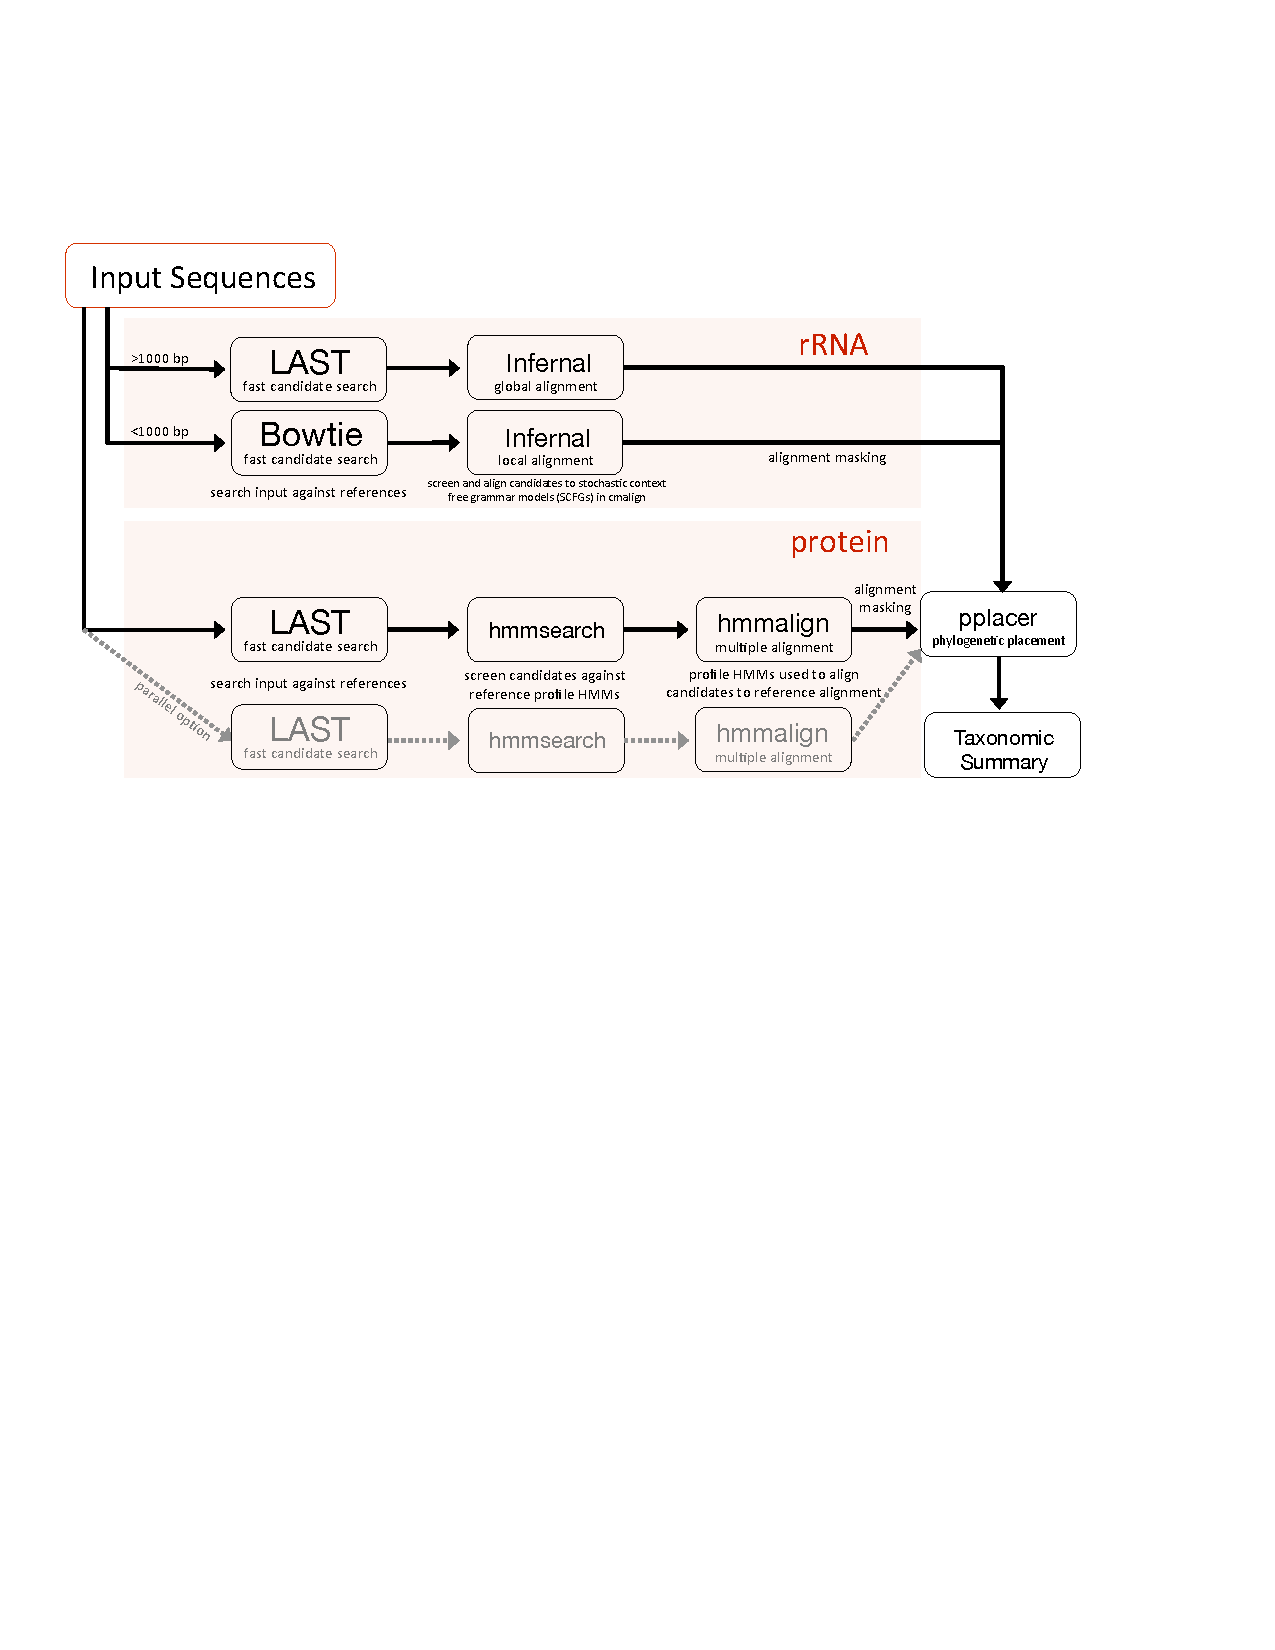
\includegraphics[trim=0 5.25in 0.5in 1.25in,clip,width=6.5in]{figures/Phylosift_overview_vector.pdf}
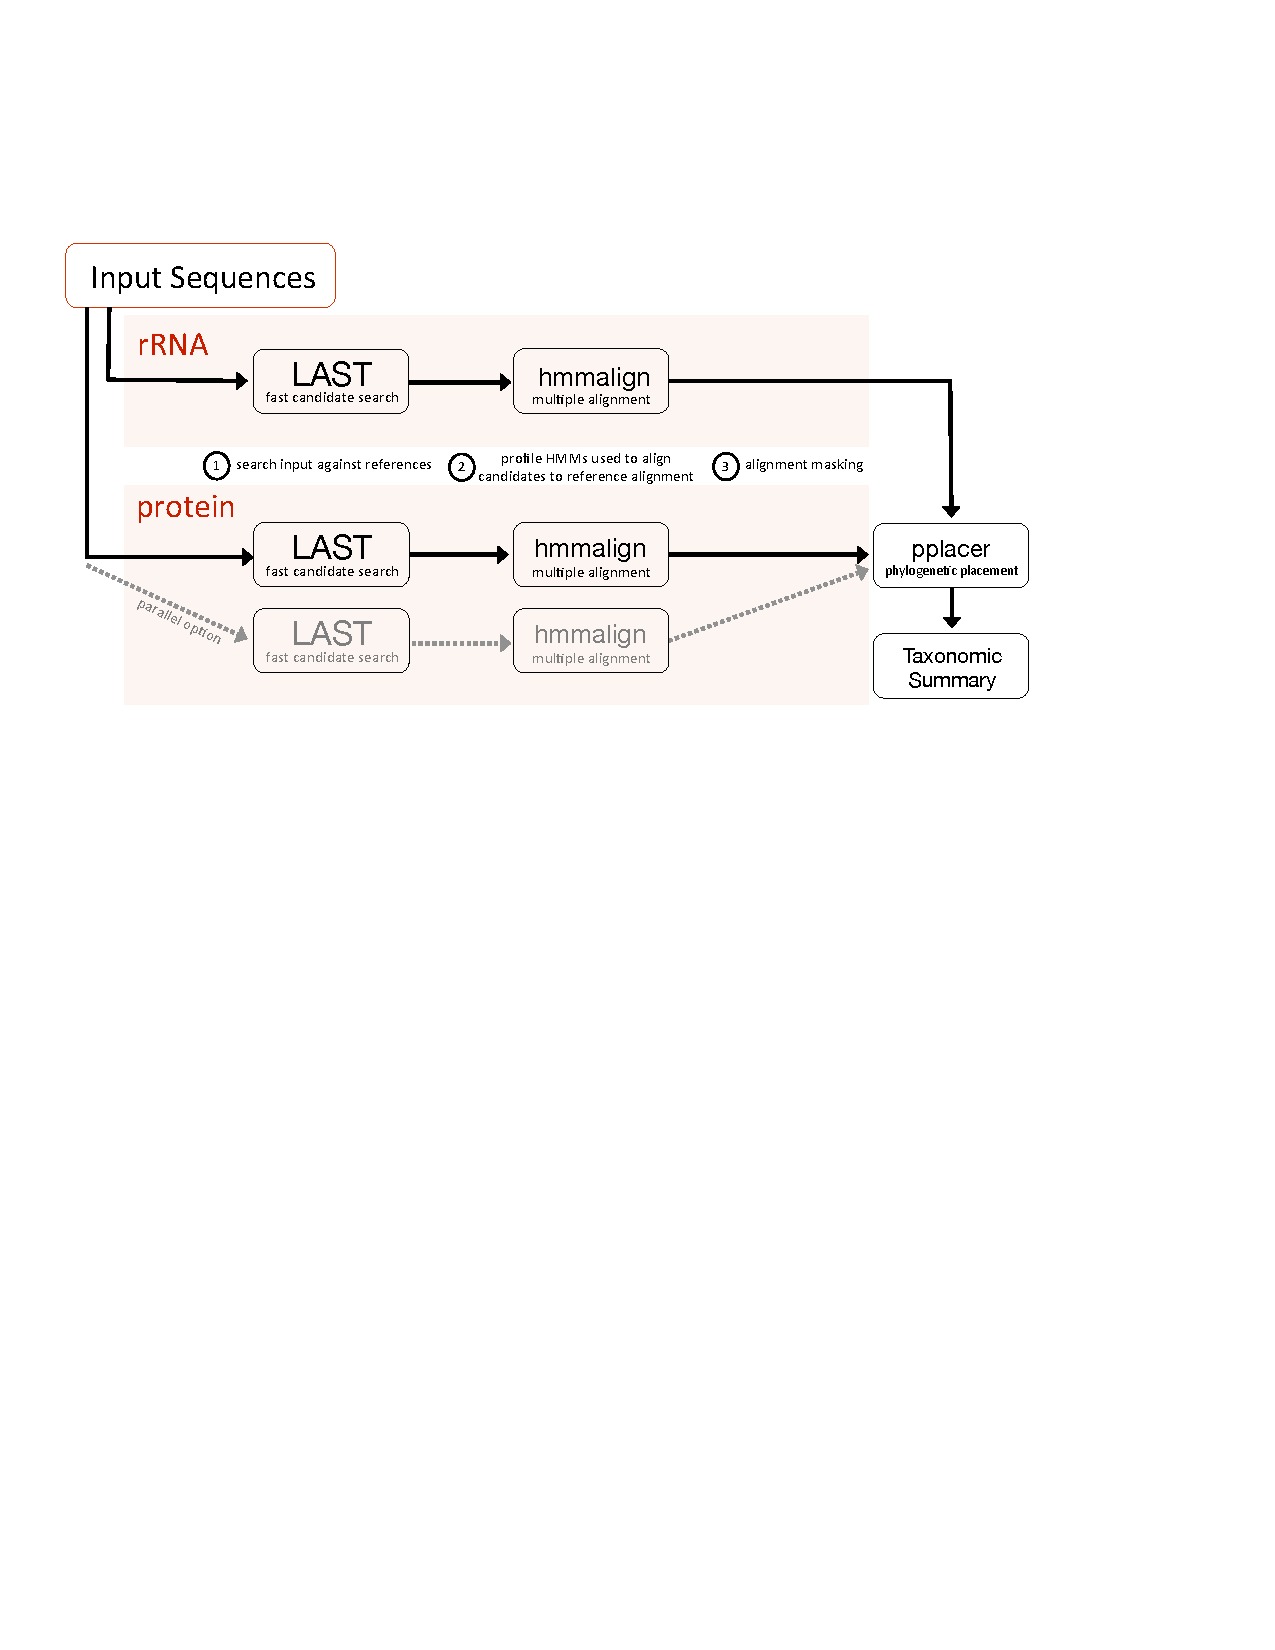
\includegraphics[width=6.5in]{figures/Phylosift_overview_oct2012_vector.pdf}
\end{center}
\caption{\textbf{PhyloSift client workflow.} This workflow is applied to the user's sequence data. DNA input sequences are processed via both the rRNA and protein parts of the workflow.}
\label{fig:overview}
\end{figure}

\begin{figure}[hp]
\begin{center}
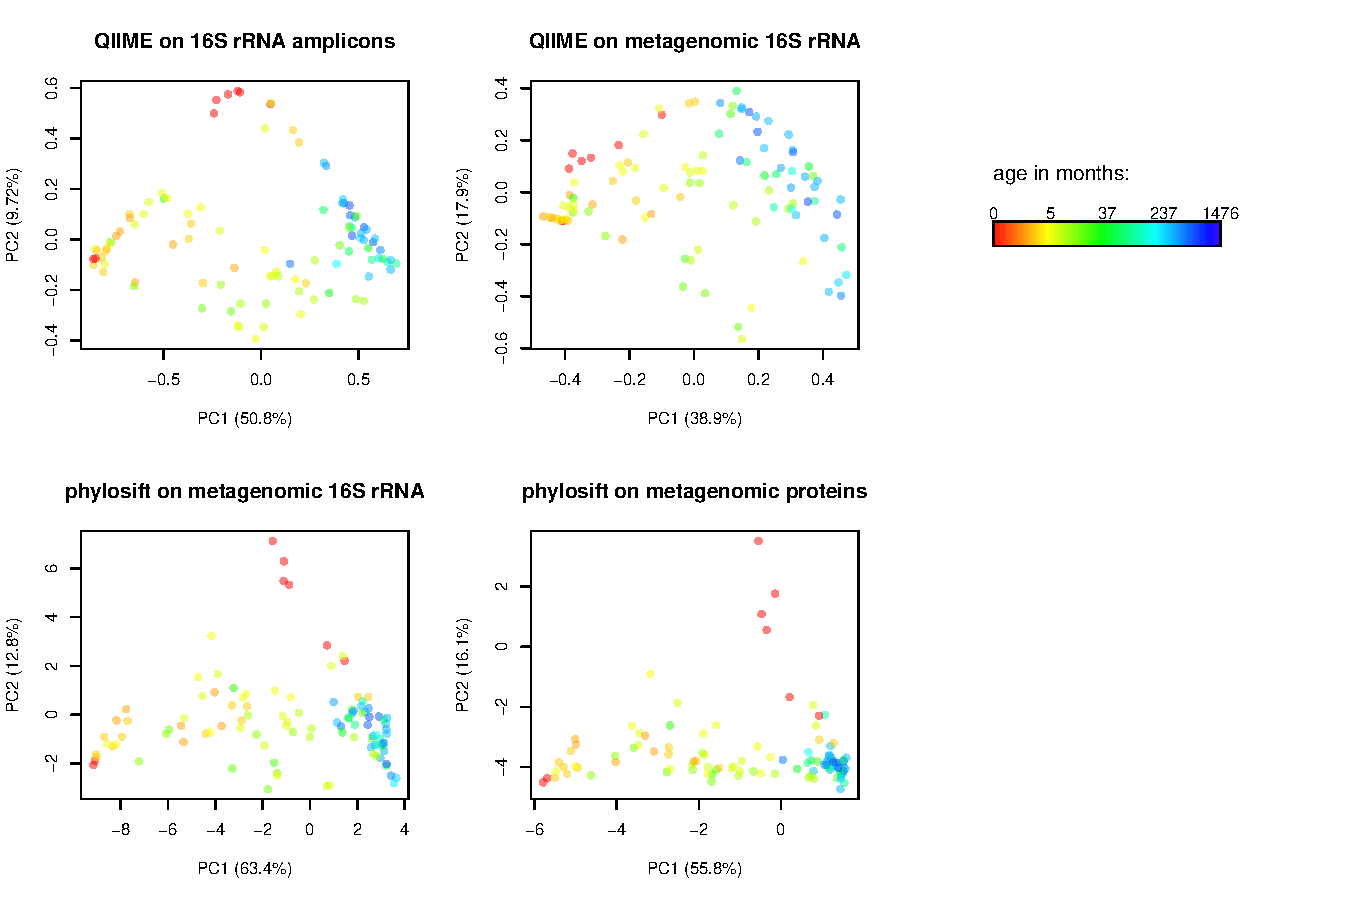
\includegraphics[width=6in]{figures/allofem.pdf}
\end{center}
\caption{\textbf{Comparison of QIIME PCA and edge PCA analysis of human fecal samples.} Samples from 106 individuals were analyzed by PCA to evaluate trends in community composition with respect to host age. 16S rDNA amplicon data and metagenomic data from the same samples was processed using QIIME and PhyloSift. QIIME analyzed the amplicon data (top left) and 16S rDNA reads extracted from the metagenomic data (top right) using a reference-based OTU picking strategy. PhyloSift analyzed the same metagenomic 16S rDNA reads (bottom left) and reads matching the 40 elite gene families (bottom right). Each PCA approach gives qualitatively similar results.}
\label{fig:agepca}
\end{figure}

\begin{figure}[hp]
\begin{center}
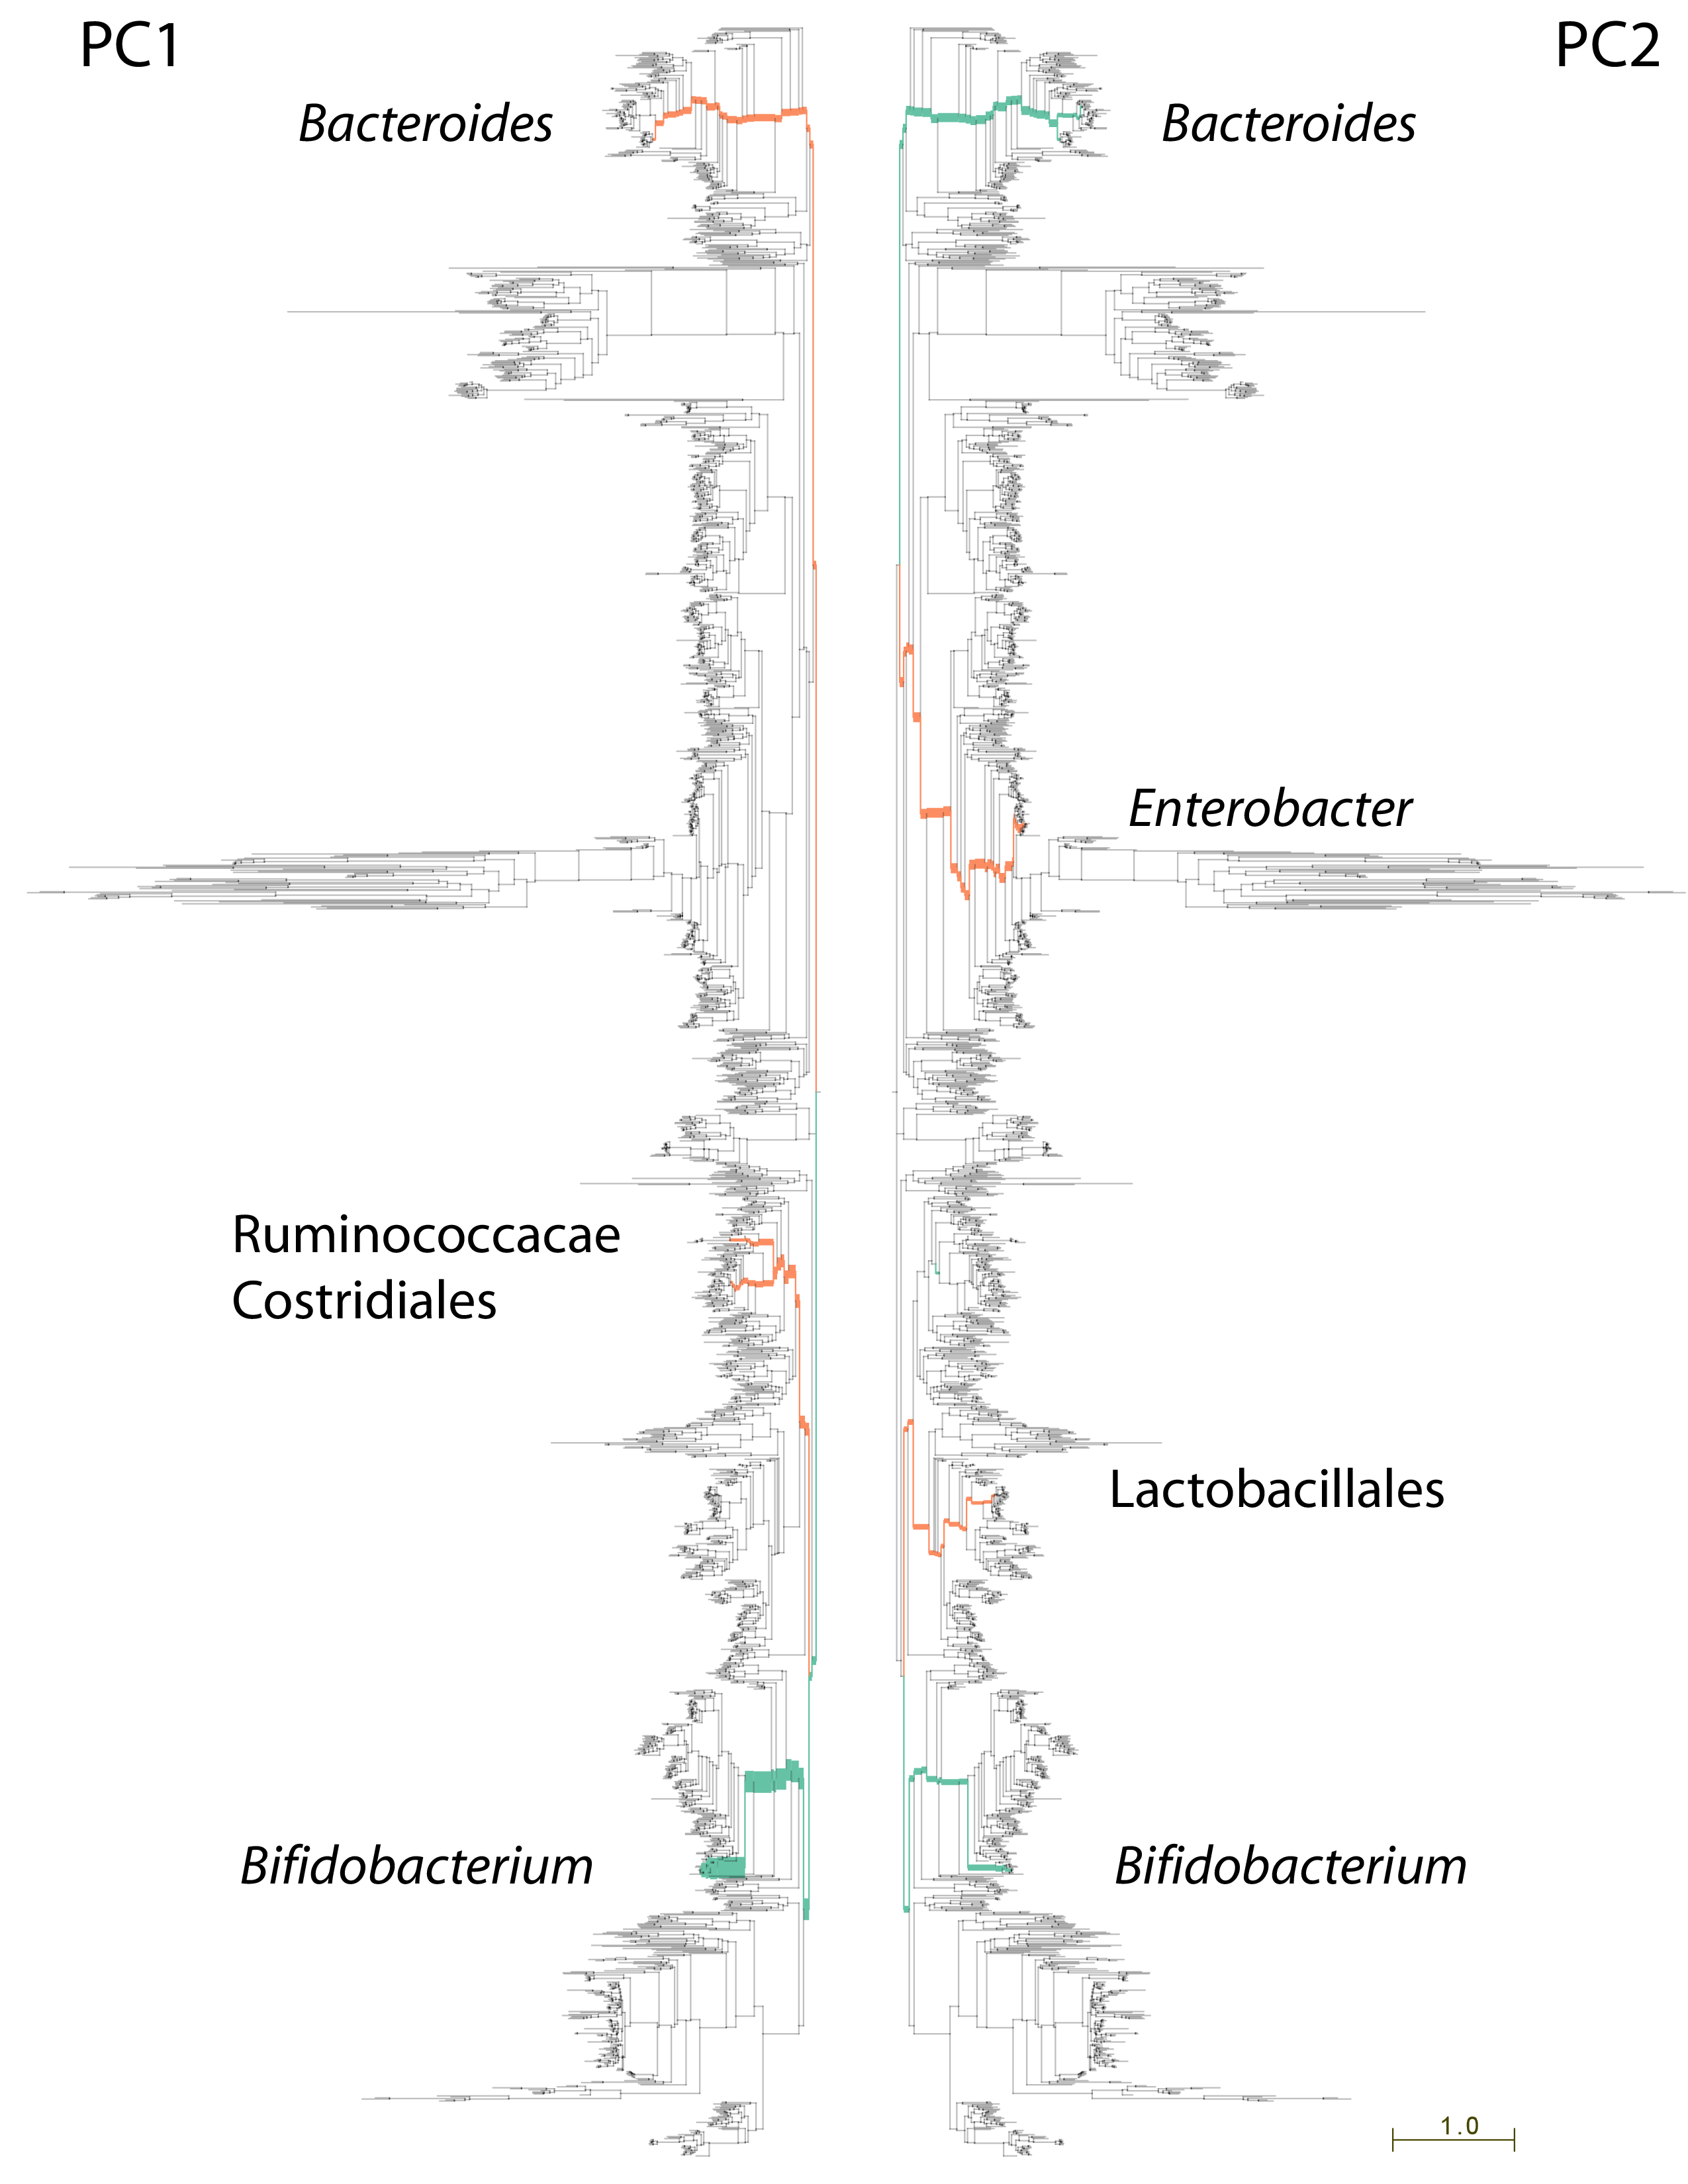
\includegraphics[width=6in]{figures/both_prettylike_b2b.png}
\end{center}
\caption{\textbf{Lineages contributing variation in human fecal sample community structure.} 106 metagenomic samples were processed using PhyloSift and their community composition compared using Edge PCA~\cite{Matsen2012}. Lineages that decrease in abundance along the principal component axis are shown in turquoise color, those increasing in abundance are shown in red. Edge width is proportional to the change in abundance. Remaining lineages in the phylogeny of bacteria, archaea, eukarya, and some viruses are shown in light gray. PC1 shown at left, PC2 at right.}
\label{fig:pcaphylo}
\end{figure}

\begin{figure}[hp]
\begin{center}
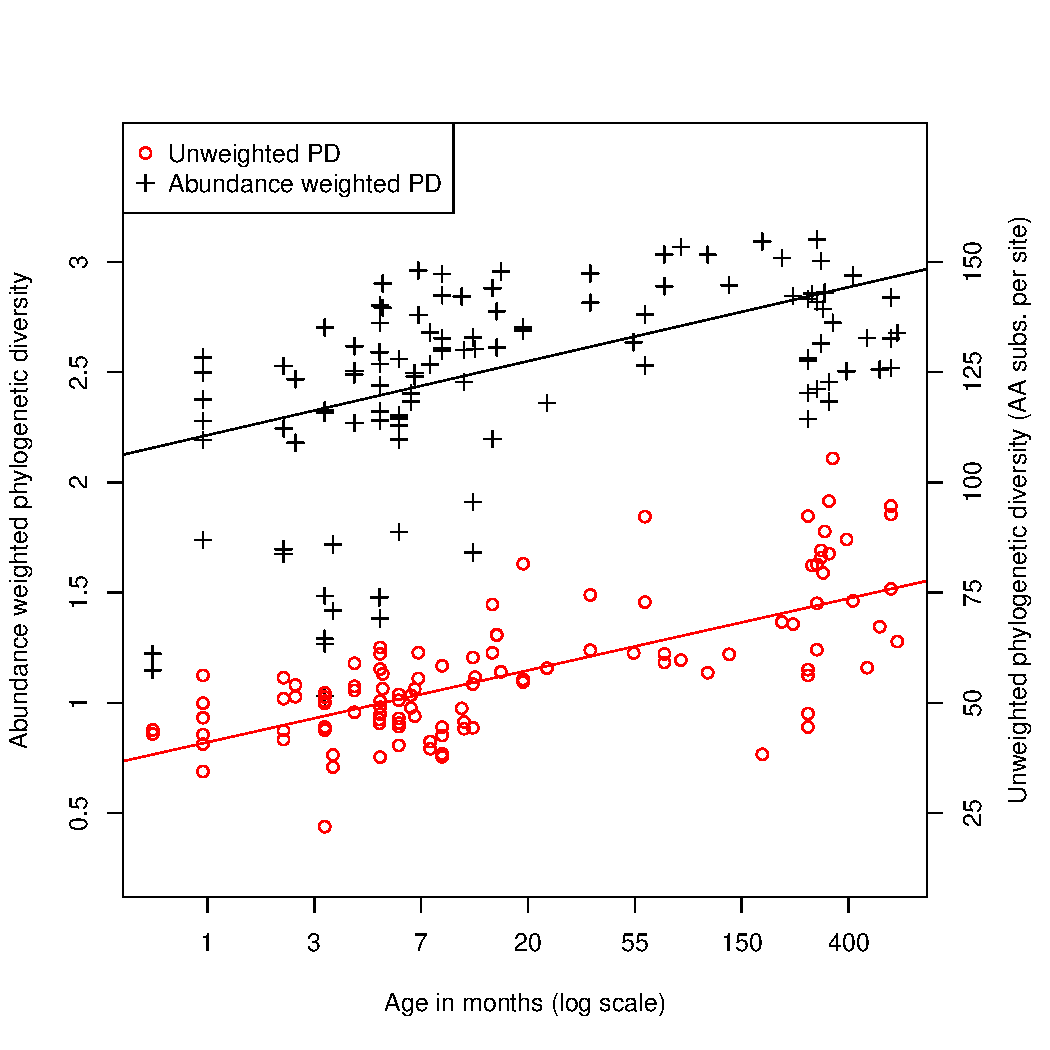
\includegraphics[width=4in]{figures/phylo_diversity.pdf}
\end{center}
\caption{\textbf{Relationship betwen fecal community phylogenetic diversity and host age.} 106 metagenomic samples were processed using PhyloSift and their phylogenetic diversity analyzed using two metrics. Unweighted phylogenetic diversity (PD) simply measures the total branch length of the reference tree covered by placed reads from a sample. Balance-weighted phylogenetic diversity adjusts these values by the abundance of each lineage in the sample. In unweighted PD, a log-linear relationship between host age and fecal community phylogenetic diversity can be observed. Balance weighted PD, on the other hand, shows rapid growth in early life followed by slow decline after the first year, consistent with a small number of  divergent lineages becoming dominant in the fecal ecosystem.}
\label{fig:agediversity}
\end{figure}

\begin{figure}[hp]
\begin{center}
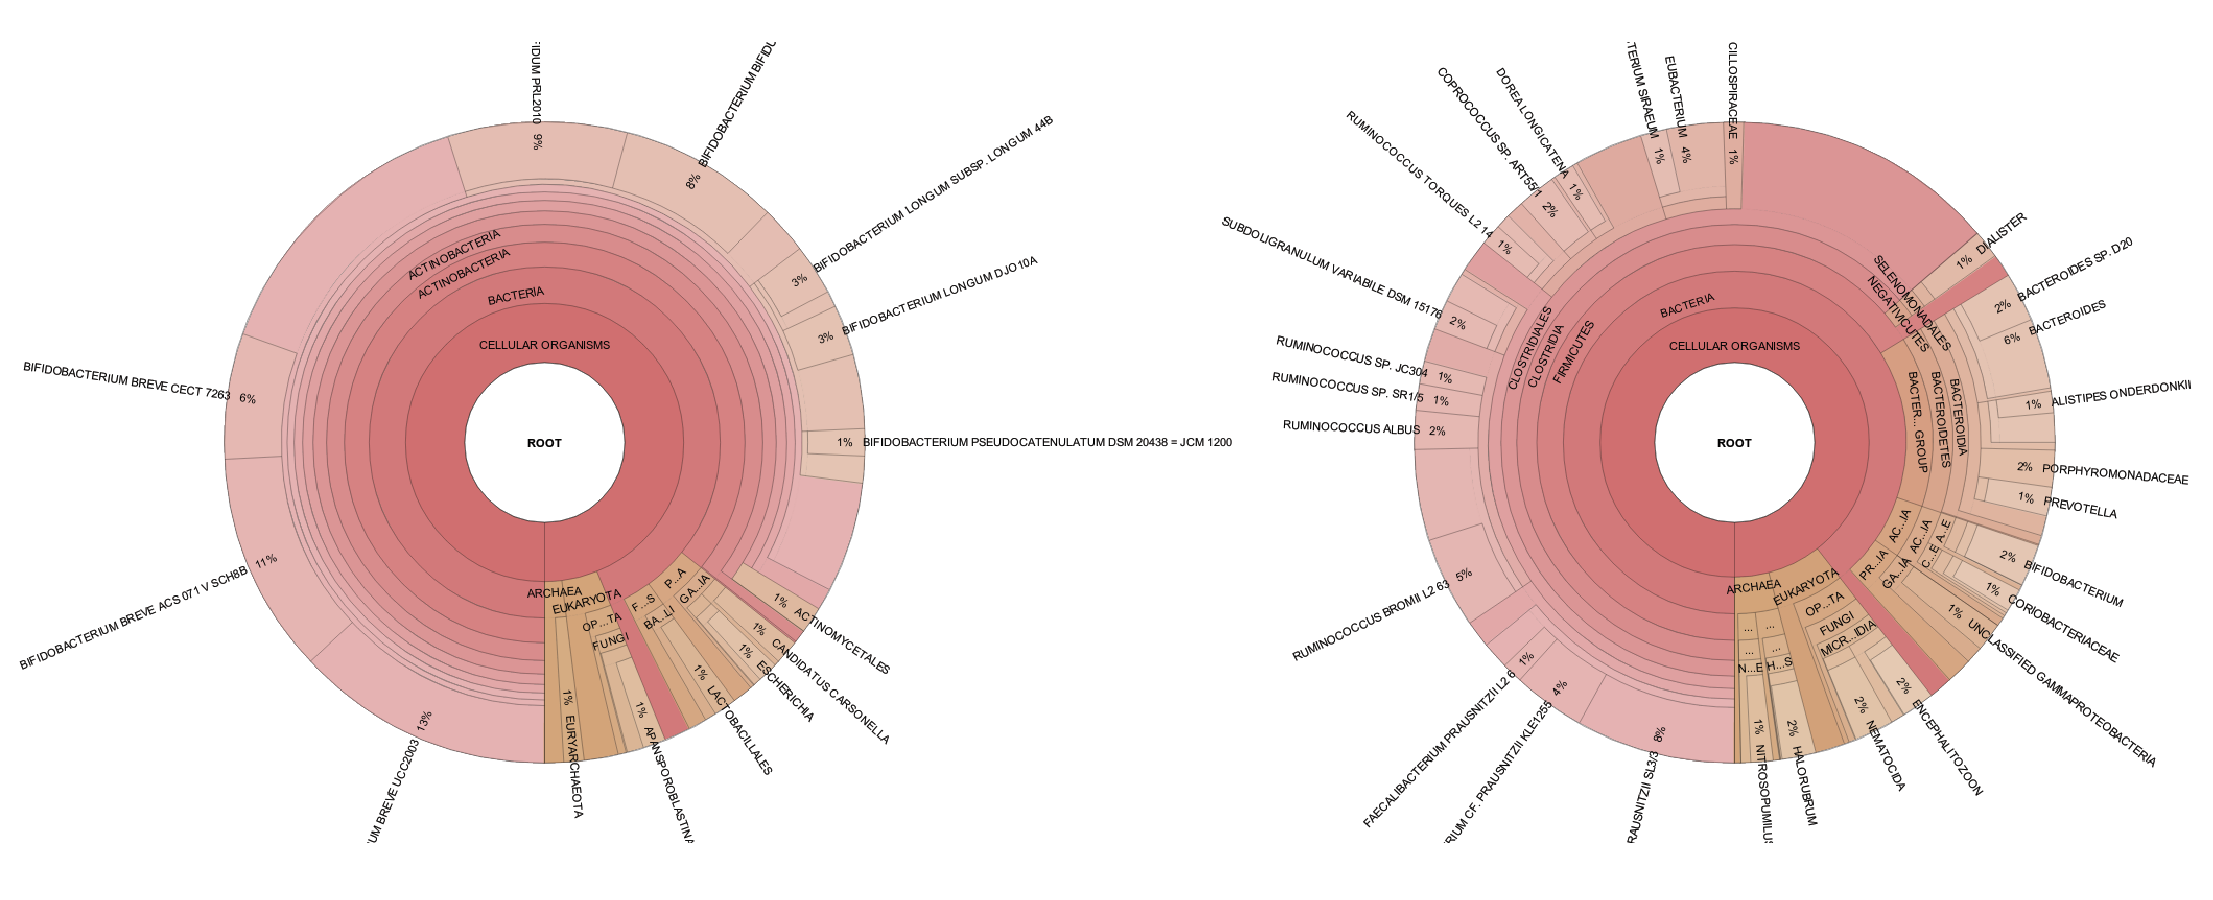
\includegraphics[width=6.5in]{figures/krona_two.pdf}
\end{center}
\caption{\textbf{Taxonomic visualization of two human gut samples.} Data analyzed by PhyloSift, visualized by Krona.}
\label{fig:kronaplots}
\end{figure}


\clearpage

\end{document}

